% Kapitel 3

\chapter{Reducing Model Input Sizes with Model-Driven Crops}
\label{chap:reducing-input-size}

In this chapter, we will present a simple but powerful way of reducing the sizes of input images to segmentation neural networks using image crops. We will show why reducing the input size can lead to an increase in data efficiency. Finally, we will evaluate the approach empirically using two similar methods on various medical image modalities.

In Chapter \ref{chap:data-efficiency} of this thesis we discussed how increasing the number of parameters of a model allows it to overfit more easily. Additionally, we discussed how more complex problems require more parameters to be modeled. Thus, for small datasets, it is beneficial to reduce the complexity of the problem to allow for using networks of fewer parameters. A simple way to reduce the complexity of problems in convolutional neural networks is to reduce the size of the images.

To understand how reducing input size reduces model complexity, let us revisit the concept of sample complexity \(n(\epsilon, \delta)\) and its established bounds \cite{shalev-shwartzUnderstandingMachineLearning2014}:
\begin{equation}
	n(\epsilon, \delta) \geq \frac{\log(\lvert \mathcal{F} \rvert / \delta)}{\epsilon},
\end{equation}
where \(n\) represents the minimum number of samples needed for a model from the hypothesis space \(\mathcal{F}\) to achieve a performance that is 'probably approximately correct'—that is, within an error margin \(\epsilon\) with a confidence level of \(1 - \delta\). It is clear from this relation that as the size of the hypothesis space expands, so does the sample complexity.

The hypothesis space refers to the set of all functions that the model is capable of approximating, encompassing every conceivable mapping from the domain \(\mathcal{D}\) to the codomain \(\mathcal{C}\). Therefore, the magnitude of the hypothesis space can be expressed as
\begin{equation}
	\lvert \mathcal{F} \rvert = {\lvert \mathcal{C} \rvert}^{\lvert \mathcal{D} \rvert}.
\end{equation}

For binary CNN-based image segmentation, the model maps \(c\)-channeled images \(I \in \mathbb{R}^{w \times h \times c}\) to binary masks \(M \in \{0, 1\}^{w \times h}\). The hypothesis space thus grows with the image dimensions \(w, h\), and the number of channels \(c\). Reducing image size directly decreases the hypothesis space, lowering the sample size needed for effective training. This relationship is supported by empirical findings --- \citet{tanEfficientNetRethinkingModel2020} show that convolutional neural networks perform best when input size, network depth, and width are scaled proportionally.

Smaller input sizes also offer technical benefits, notably reduced memory demands. Since CNN memory requirements grow exponentially with image size, larger inputs significantly limit batch size during training. This constraint not only slows down the training process but can also affect the accuracy of gradient estimates per batch, potentially destabilizing training.

The method of image scaling is crucial for performance in medical image segmentation tasks, where images are typically downscaled uniformly. This process can lead to the loss of critical fine details, such as edges, which are vital for segmentation accuracy in medical imaging. For example, the pericardium's thin structure around the heart, often less than 2 mm and represented by only a few pixels in cardiac CT scans, can be obscured or entirely lost through downsampling. This information loss is particularly detrimental for small objects, which are prevalent in medical images.

An effective way to overcome this loss of information while still reducing the image is cropping the image to a region of interest. By focusing on the area containing the target object for segmentation, the network's learning task is simplified, removing the need to filter out irrelevant background areas. Additionally, centering and uniformly scaling the object across images can further reduce the variance of the data, enabling the network to use fewer parameters. Given this, we will now propose a method to effectively use image cropping as a way of reducing neural network input size.

\section{Model-Driven Image Cropping}

We introduce a strategy to minimize the input size for segmentation networks, focusing on cropping rather than uniform downsampling. This method involves isolating each object within the original high-resolution image, cropping these areas, and performing segmentation on the individual cropped sections. By concentrating on smaller crop regions instead of the entire image, we significantly reduce the network's input size while preserving essential pixel information within the objects. This approach is illustrated in \figref{fig:summary}, providing a visual summary of the process.

\begin{figure}[b!]
\centering
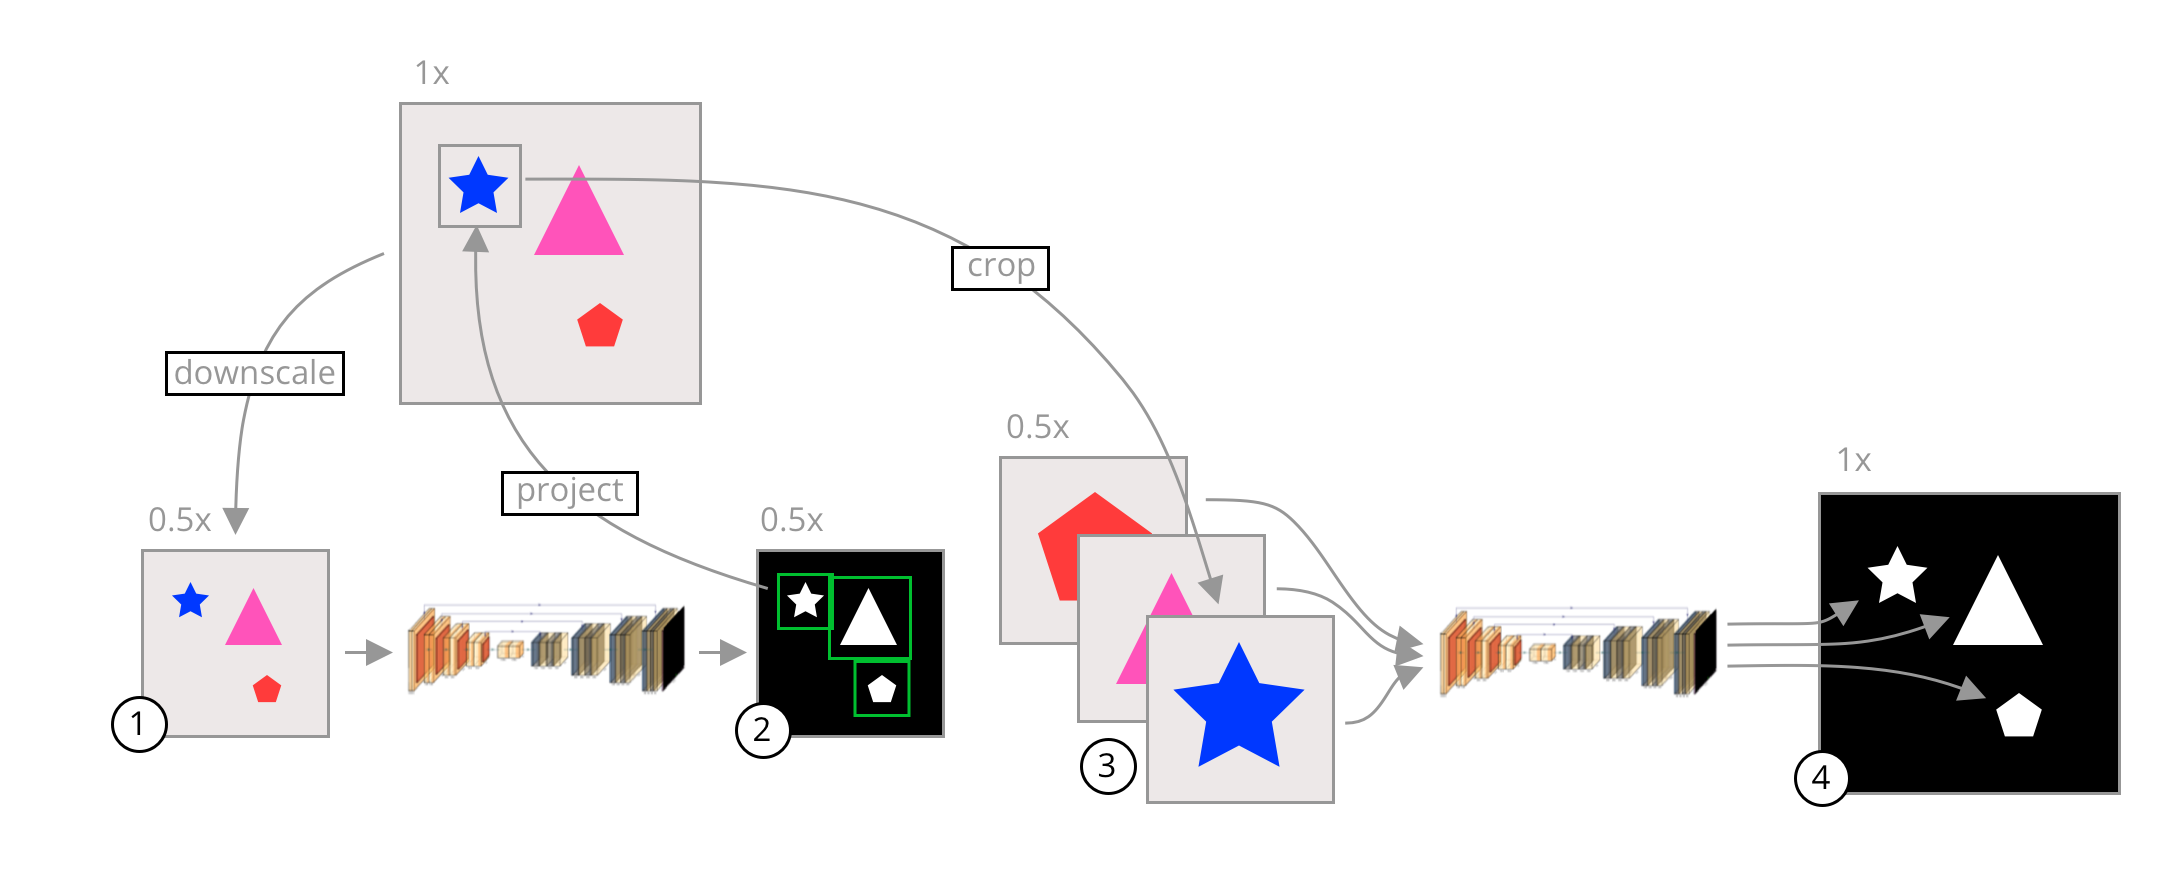
\includegraphics[width=\textwidth]{images/5/explainer-diagram.png}
\caption{A visual summary of our approach. (1) An image is uniformly downsampled from its original resolution. (2) A rough segmentation is predicted by a neural network, and the bounding box of each connected component is calculated. (3) The bounding boxes are scaled to the original image space and crops of the input image are taken in the original resolution and scaled to a common input size. (4) Each crop is segmented separately by a second neural network specifically trained on cropped images. These crops are fused to form a final segmentation in the original high resolution. \cite{bencevicSegmentthenSegmentContextPreservingCropBased2023a}\label{fig:summary}}
\end{figure}

The inference procedure using our method is as follows. Let $I$ be an input image of size $W \times H$. We obtain a rough segmentation using $M_{rough} = g_{\phi_1}(C(I))$, where $M_{rough}$ is a binary segmentation mask generated by $g_{\phi_1}$, a CNN with input and output size $S \times S$, parameterized by $\phi_1$; and $C$ is a uniform downsampling operation from  $W \times H$ to $S \times S$. 

Given $N$ connected components of $M_{rough}$, a set of bounding boxes $\{b_i\}, i \in [1..N]$ is calculated enclosing each connected component, described in more detail later in this chapter. The bounding boxes are used to generate a set of crops $\{I_i: I_i = I(T_i(b_i))\}$, where $T_i$ is a scaling and translation of the bounding box in $S \times S$ space to the corresponding region in the $W \times H$ space.
The crops are used to generate a set of fine segmentation masks $Y_f$ using:
\begin{equation}
Y_f = \{Y_{fi}: Y_{fi} = g_{\phi_2}(C_i(I_i)), i \in 1..N\},
\end{equation}
where $g_{\phi_2}$ is a CNN of the same architecture as $g_{\phi_1}$ and size $S \times S$, parameterized by $\phi_2$, and $C_i$ is a scaling operation from the width and height of $I_i$ to $S \times S$. A final segmentation $y$ is formed using:
\begin{equation}
y = max(\{(T_i \circ C^{-1}_i)(Y_{fi}), i \in 1..N\}),
\end{equation}
where $y$ is the resulting segmentation formed as the maximum value in all of the fine segmentations, transformed to their corresponding regions in $W \times H$ space. This process is described in more detail in Algorithm \ref{alg:crop}. 

The rough segmentation network $g_{\phi_1}$ is trained on uniformly downsampled images. The network outputs a rough, low-resolution segmentation mask. The rough segmentation mask contains a number of connected components. For each connected component, we calculate a bounding box that encompasses all of its pixels. These bounding boxes are the crop regions used for the fine segmentation network. Since we only use this segmentation to obtain rough regions of interest, the input images to this network can be heavily downsampled without impacting the final fine segmentation.

The fine segmentation network $g_{\phi_2}$ is trained on cropped images using the ground truth segmentation masks to generate the bounding boxes. This network produces a fine segmentation of that region of the image. Since we know the original bounding box of each crop, we can resize the final segmentation to its original size and translate it to its original position. We perform this for each object in the image, fusing each of the fine segmentation masks into a final segmentation mask in the original image resolution.

In other words, our method performs zooming and panning around the original image and builds a final segmentation piece-wise from each zoom and pan. This allows us to use neural networks with very low input sizes without requiring a large amount of downscaling. What follows is a detailed description of the different parts of the segmentation process.

\begin{algorithm}
\caption{Inference algorithm for one input image}\label{alg:crop}
\begin{algorithmic}
 \renewcommand{\algorithmicrequire}{\textbf{Input:}}
 \renewcommand{\algorithmicensure}{\textbf{Output:}}
\Require High-resolution input image $I$ of size $H \times W$, \\
         input size $S$, padding $k$, \\
		 neural network NET\_1 trained in $S \times S$ downscaled images, \\
		 neural network NET\_2 trained on ground truth $S \times S$ image crops.
\Ensure Output image $Y$ of size $H \times W$.
\\
\State $I' \gets \Call{resize}{I, (S, S)}$
\State $y' \gets \Call{net\_1}{I'}$
\State $y' \gets \Call{resize}{y', (H, W)$}
\State $ccs \gets \Call{connected\_components}{y'}$
\State $crops \gets [ ]$ \Comment{An array of $S \times S$ images}
\State $bboxes \gets [ ]$ \Comment{An array of bounding boxes for each crop}
\\
\For{cc in ccs}
	\State $bbox \gets bounding\_box(cc)$
	\State $bbox.width \gets bbox.height \gets \Call{max}{bbox.width, bbox.height}$
	\State $bbox \gets (bbox.left - k, bbox.top - k, bbox.width + k, bbox.height + k)$
	\State $bbox \gets \Call{shift\_to\_image\_region}{bbox, (H, W)}$
	\State $crops.\Call{add}{\textsc{crop}(I, bbox)}$
	\State $bboxes.\Call{add}{bbox}$
\EndFor
\\
\For{crop, i in crops}
	\State $l, t, w, h \gets bboxes[i]$
	\State $crop \gets \Call{resize}{crop, (S, S)}$
	\State $y_{crop} \gets \Call{net\_2}{crop}$
	\State $y_{crop} \gets \Call{resize}{y_{crop}, (h, w)}$
	\State $Y[t:t+h, l:l+w] \gets Y[t:t+h, l:l+w]\ ||\ y_{crop}$
\EndFor
\end{algorithmic}
\end{algorithm}

\subsubsection{Cropping}\label{cropping}

The key to reducing downscaling in our approach is that we take crops from the image in the original resolution. The crop regions themselves are predicted on a downscaled image and then projected to the original image space.

The cropping procedure is as follows. First, a bounding box fully encompassing each connected component in the rough segmentation is calculated. The coordinates of the bounding box are then scaled to the high-resolution image space. An empirically determined padding of $S/8$ (for an $S \times S$ input size) is added along each of the four sides. This way of cropping preserves the context of the object and decreases the number of false negatives inside the bounding box.

The box is then squared, i.e. its height and width are set to the larger of the two dimensions. The box is also shifted (maintaining its width and height) to be fully inside the region of the image. Finally, the bounding box is used as a region to crop the original high-resolution image. The rough segmentation sometimes results in noisy regions, so each crop whose width or height is less than 5 pixels is discarded.

\pagebreak

\subsubsection{Fine Segmentation and Fusion}

Each crop of the high-resolution image is scaled to the input size of the fine segmentation network. The fine segmentation network outputs a number of segmentation masks equal to the number of connected components in the rough segmentation. A high-resolution segmentation mask is created by translating and scaling each of the fine segmentation network outputs to their original position. By doing so we construct a full segmentation piece by piece, where each piece is a fine segmentation of a single object in the image, as detected by the rough segmentation. If the cropped regions overlap in the final segmentation, we use a logical \verb|OR| operator to resolve the conflict in the fine segmentation mask. This process is presented in Algorithm \ref{alg:crop}.

\subsubsection{Training the Fine Segmentation Network}

The fine segmentation network is trained on ground truth image crops. The crops are obtained by using the connected components of ground truth segmentation masks. From there, the crops are prepared in the same way as described above. Since the images have multiple crop regions, we choose one of the crop regions of the full-resolution image at random during each training iteration. If the original image has no connected components in the ground truth segmentation mask, the whole image is used as training input. All input images to the fine segmentation network are resized to $S \times S$, where $S$ is a pre-determined input size that matches the input size used to train the rough segmentation network.

During training, we add an augmentation step by adding random noise to the crop region. When preparing the crops during training, a uniformly distributed random number between $\pm16$ pixels is added to each dimension of the bounding box (the $x$- and $y$-coordinate, width, and height). This ensures that the trained network is robust to imperfect rough segmentation masks during inference.

In our experiments, we used the same architecture for both the rough and fine segmentation networks, as this allows us to use transfer learning. However, there is no requirement that the networks use the same architecture.

\subsection{Related work}

The approach presented in this chapter is motivated partly by the work of \citet{Qiu2018}, where a dataset of images is manually cropped to the object boundary, leading to an increase in segmentation performance. This was applied to skin lesions where it achieved a scale-unifying effect across the dataset. In this chapter, we adapt this approach to use a neural network to predict the optimal object boundary and develop specific ways to train the fine segmentation network on cropped images. In addition, we allow for taking multiple crops on the image and later fusing them in the final segmentation, which makes the method applicable to a wider range of segmentation tasks.

 In the previous chapter, a related approach is presented using the polar transform as a pre-processing step. The main novelty in this chapter is the use of cropping as a transformation step. The rest of the approach was then adapted to better suit a cropping transformation, including bounding box augmentation and padding the bounding box. This allows our approach to be used to reduce the input size of the networks.
 
\subsubsection{Detect-then-segment}

Several recent end-to-end neural network architectures for segmentation incorporate cropping in one of their layers \cite{girshickRichFeatureHierarchies2014, heMaskRCNN2017}. These generally use object detection to find a region of interest which is then segmented. This approach can be called \textit{detect-then-segment}. In models such as R-CNN \cite{girshickRichFeatureHierarchies2014} the objects are first detected and then fed into the segmentation pipeline. Mask R-CNN \cite{heMaskRCNN2017} uses object detection to extract a region of interest in the feature masks within the network. These methods effectively concentrate the network on a region of the image. However, information is still lost if the images are uniformly downsampled as a preprocessing step. In contrast, our approach allows one to use low input sizes by cropping the image before it enters the network. Compared to \textit{detect-then-segment} approaches, cropping as a preprocessing step reduces the number of parameters while increasing the pixel-level information in the salient regions of the image. In addition, our approach leads to rescaling each object to the same size before the fine segmentation, which increases the scale-invariance of the models.

\subsubsection{Coarse-to-fine Segmentation}

Our approach can be described as a coarse-to-fine approach to image segmentation. There have been similar approaches to medical image segmentation. \citet{zhouFixedPointModelPancreas2017} describe an approach to pancreas segmentation using a fixed-point model \cite{pmlr-v28-li13b}. They train a coarse and a fine segmentation network. The coarse network obtains an initial region of the pancreas which is then re-segmented using the fine network. The fine network then re-segments its output again, and this process is repeated iteratively until a stable solution emerges. They also use bounding box augmentation during training. Our approach differs in two ways. Firstly, we only use one iteration at a stable input size, improving the inference time. Secondly, our approach supports segmenting multiple objects on the image.

\citet{zhu3DCoarsetoFineFramework2018} describe an approach to pancreas segmentation with two neural networks. The first network is a coarse segmentation network trained on overlapping 3D regions of the whole CT volume. The second network is a fine segmentation network that is trained on only the regions where the ground-truth images contain the pancreas. During inference, the fine network re-segments densely overlapping regions of the rough segmentation. The main difference in our approach is the use of only one region of interest per object where the whole object is visible and uniform in scale. This allows us to use networks of a lower capacity while still maintaining good segmentation results.

Similarly to our approach, \citet{jhaInstanceSegmentationWhole2021} split the segmentation process into detection and segmentation stages. They use a neural network to first detect an object in a downsampled image. They then use the bounding box to crop the object in the high-resolution image. Our approach differs in several ways. Firstly, our approach allows the detection of multiple objects on the image and describes a way to fuse the segmentations of different objects. Secondly, we present new ways to train the fine segmentation network to make the fine segmentation network more robust to imperfect bounding boxes. Finally, we propose a generalized approach evaluated on a variety of different modalities of medical images.

\subsubsection{Non-uniform Downsampling}

The resolution of an input image for neural networks can be reduced using a more complex sampling strategy. \citet{marinEfficientSegmentationLearning2019} use non-uniform downsampling for this task. Their approach consists of training a neural network to sample points near object boundaries. The sampling points are then used to downsample the image and perform a final segmentation using a second neural network trained on the downsampled images. Similarly, \citet{jin2022learning} use a learnable deformable downsampling module which is trained together with a segmentation module end-to-end. Our approach differs in the use of cropping instead of non-uniform downsampling, which preserves the topology of the image and provides localization of the object.

\subsubsection{Other Approaches to Reducing Input Resolution}

Recently, transformer-based architectures such as SegFormer \cite{xie2021segformer} and the Swin Transformer \cite{liu2021Swin} have become popular approaches to semantic segmentation. These networks are trained on a large number of small, overlapping patches of the image. The network uses self-attention to determine the saliency of each patch. In a sense, this allows the network to be trained on very small input image dimensions. However, transformers require a very large amount of data to be trained and have large memory requirements \cite{dosovitskiy2020vit}, so their use is currently limited in the domain of training on downscaled medical images.

For whole slide images, the input size is often reduced by dividing the image into equally sized patches \cite{nazeriTwoStageConvolutionalNeural2018, houPatchBasedConvolutionalNeural2016}. A downside of this approach is computational complexity during inference since not all patches are relevant. Additionally, errors can arise when the objects are split by the patch boundary.

%%%%%%%%%%%%%%%%%%%%%%%%%%%%%%%%%%%%%%%%%%
\subsection{Results}

We evaluate our approach on three separate datasets, hereafter referred to as the cells, aorta, and polyp datasets. First, for each dataset, we trained a rough segmentation U-Net, Res-U-Net++, and DeepLabv3+ network at various downscaled input resolutions. These models are also used as baseline models to compare against our approach. To evaluate our approach, we train fine segmentation models using the same combinations of datasets, architectures, and input sizes. 

Altogether more than 100 neural networks were trained to evaluate our approach, including both the baseline networks and networks trained on cropped images.

Each network is trained from scratch using the downscaled dataset. The outputs from the networks are then upscaled to the datasets' original resolution, and the metrics are calculated using those outputs. We use the held-out test datasets for all of the results reported in this section. The baseline models are used as the rough segmentation networks for the experiments using our approach. The hyperparameters used for each network are reported in Table \ref{tab:hyperparams}.

In the interest of providing objective metrics of model performance, all of the hyperparameters were tuned using the validation dataset on the baseline U-Net. Those same hyperparameters are then used for each of the models in our approach. Each model is trained using the Adam optimizer up to a maximum number of epochs and the best model with the best validation loss is saved during training. The validation loss is calculated as the Dice score coefficient (DSC) over the validation dataset at the same resolution as the input images. We do not upscale the outputs for the validation loss as we do for calculating the final metrics. Each model was trained using PyTorch 1.10 on an Nvidia GeForce RTX 3080 GPU. Where possible, we have fixed the random seed value an arbitrarily chosen value of ``2022'', but we have also run the experiments on two other random seeds and obtained similar results. Other hyperparameters were chosen based on validation DSC.

\begin{table}[t!]
\caption{The hyper-parameters used for each of the models in our experiments.\label{tab:hyperparams}}
\newcolumntype{C}{>{\centering\arraybackslash}X}
\begin{tabularx}{\textwidth}{CCCC}
\textbf{Dataset} & \textbf{Batch size} & \textbf{Learning rate} & \textbf{Max. epochs} \\
\midrule
Cells & 16 & $5 \cdot 10^{-4}$ & 100\\
Polyp & 8 & $10^{-3}$ & 175\\
Aorta & 8 & $10^{-3}$ & 100\\
\end{tabularx}
\end{table}
\unskip

\subsubsection{Datasets}\label{datasets}

This section briefly describes the datasets used in our experiments as well as the preprocessing steps for the images. For more details, we direct readers to the supplemental code repository available at \href{https://github.com/marinbenc/segment-then-segment}{github.com/marinbenc/segment-then-segment}. To evaluate our approach, we chose three datasets across different medical imaging modalities, including CT scans, microscopy imaging, and colonoscopy images. We hope that the variety in the datasets will show the generalizability of our approach. Aside from the variety, the datasets were selected because they include images of large dimensions on which small objects of various sizes need to be segmented. These types of tasks are most likely to suffer from the loss of information due to downscaling and are thus particularly suitable to be segmented using our approach.

\textbf{Aorta Dataset}: For aorta segmentation we use the AVT dataset \cite{radlAVTMulticenterAortic2022}, a multi-center dataset of labeled CTA scans of the aortic vessel tree. We only use a subset of the dataset from Dongyang Hospital, a total of 18 scans of between 122 and 251 slices. Each slice is windowed to 200 to 500 HU, normalized to $[-0.5, 0.5]$, and zero-centered by subtracting 0.1 from each slice. The original resolution of the slices is $512 \times 666$ pixels. We use augmentation during training. Each input has a 50\% chance of an affine transform (translation of $\pm6.25\%$, scaling of $\pm10\%$, rotation of $\pm14^{\circ}$), as well as a 30\% chance of a horizontal flip. The dataset is split per patient into a training set (12 scans), validation set (3 scans), and test set (3 scans).

\textbf{Cells Dataset}: For cell nucleus segmentation we use the 2018 Data Science Bowl dataset, otherwise known as image set BBBC038v1 from the Broad Bioimage Benchmark Collection \cite{caicedoNucleusSegmentationImaging2019}. We use 670 RGB images and their corresponding labels from the \verb|stage1_train| repository. The original files are of various sizes ranging from $256 \times 256$ to $1024 \times 1024$ pixels. We did not further split the images into patches, all training is done on the whole images. We use the same augmentation as for the aorta dataset. The dataset is split into a training set (80\%, 536 images), validation set (10\%, 67 images), and test set (10\%, 67 images).

\textbf{Polyp Dataset}: For polyp segmentation, we use the Kvasir-SEG dataset \cite{jha2020kvasir}, which contains 1000 annotated gastroscopy images containing polyps. The size of the original images ranges from 332 to 1920 pixels in width. We split the dataset into train (80\%, 800 images), validation (10\%, 100 images), and test (10\%, 100 images) datasets.

\subsubsection{Quantitative Assessment}

The results of our experiments are shown in Table \ref{tab:seg-then-seg-results}. Our approach, using low input sizes, results in segmentation DSC on par or better than baseline models trained on larger input sizes using downscaled images. This is especially apparent at large downscaling factors of 4 and more, where the baseline models quickly deteriorate in their performance but our models were still able to achieve results that are close to those on full-size images. The biggest improvement is seen in terms of recall. For instance, on the 4x downscaled cells dataset, our approach leads to a 4.3 times larger recall. Likewise, for the polyp images, the recall improves from 0.039 to 0.799, a 20 times improvement. Recall is especially important in medical image segmentation since the cost of false negatives can often far outweigh the cost of false positives.

\begin{table}[t!]
\caption{The results of our approach using U-Net as the underlying architecture. The U-Net results are based on uniformly downscaled images.\label{tab:seg-then-seg-results}}
		\newcolumntype{C}{>{\centering\arraybackslash}X}
		\begin{tabularx}{\textwidth}{lCCCC}
			& \textbf{DSC [\%]} & \textbf{IoU [\%]} & \textbf{Prec. [\%]} & \textbf{Rec. [\%]}\\
			\toprule
\toprule
\textbf{Cells} ($256 \times 256$) & & & & \\
\midrule
$64 \times 64$ - U-Net & $75.70 \pm 11.82$ & $62.13 \pm 13.29$ & $75.27 \pm 12.61$ & $76.79 \pm 12.70$ \\
$64 \times 64$ - Ours & $84.28 \pm 12.83$ & $74.50 \pm 15.45$ & $84.75 \pm 14.85$ & $86.22 \pm 13.25$ \\
\midrule
$128 \times 128$ - U-Net & $84.52 \pm 10.34$ & $74.33 \pm 13.05$ & $85.21 \pm 11.61$ & $84.66 \pm 11.61$ \\
$128 \times 128$ - Ours & $84.54 \pm 9.64$ & $74.26 \pm 12.73$ & $83.97 \pm 13.00$ & $86.86 \pm 9.39$ \\
\midrule
$256 \times 256$ - U-Net & $87.62 \pm 13.55$ & $79.75 \pm 15.46$ & $89.44 \pm 14.09$ & $86.58 \pm 14.83$ \\
$256 \times 256$ - Ours & $84.91 \pm 12.65$ & $75.24 \pm 13.92$ & $83.52 \pm 14.50$ & $87.53 \pm 13.76$ \\
\bottomrule \\
\toprule
\textbf{Polyp} ($256 \times 256$) & & & & \\
\midrule
$64 \times 64$ - U-Net & $81.76 \pm 18.81$ & $72.40 \pm 21.00$ & $83.94 \pm 21.36$ & $84.84 \pm 17.30$ \\
$64 \times 64$ - Ours & $83.82 \pm 19.91$ & $75.90 \pm 22.51$ & $86.32 \pm 21.87$ & $86.72 \pm 17.84$ \\
\midrule
$128 \times 128$ - U-Net & $82.86 \pm 20.72$ & $74.75 \pm 23.32$ & $83.30 \pm 22.73$ & $88.93 \pm 17.50$ \\
$128 \times 128$ - Ours & $81.36 \pm 26.57$ & $74.58 \pm 27.52$ & $82.49 \pm 27.55$ & $85.23 \pm 25.33$ \\
\midrule
$256 \times 256$ - U-Net & $83.80 \pm 16.08$ & $74.88 \pm 20.44$ & $87.91 \pm 19.29$ & $84.37 \pm 16.55$ \\
$256 \times 256$ - Ours & $84.68 \pm 19.40$ & $77.11 \pm 22.53$ & $87.10 \pm 20.91$ & $87.42 \pm 18.41$ \\
\bottomrule \\
\toprule
\textbf{Aorta} ($256 \times 256$) & & & & \\
\midrule
$128 \times 128$ - U-Net & $81.03 \pm 14.45$ & $70.13 \pm 17.02$ & $85.09 \pm 14.14$ & $78.30 \pm 15.04$ \\
$128 \times 128$ - Ours & $88.50 \pm 11.08$ & $80.73 \pm 13.93$ & $92.42 \pm 10.33$ & $86.02 \pm 12.25$ \\
\midrule
$256 \times 256$ - U-Net & $72.30 \pm 28.69$ & $62.97 \pm 28.74$ & $91.21 \pm 25.39$ & $63.80 \pm 29.11$ \\
$256 \times 256$ - Ours & $80.10 \pm 25.18$ & $72.12 \pm 25.74$ & $86.75 \pm 24.14$ & $76.39 \pm 26.51$ \\
\midrule
$512 \times 512$ - U-Net & $89.34 \pm 14.59$ & $83.10 \pm 18.26$ & $96.03 \pm 11.52$ & $85.66 \pm 17.44$ \\
$512 \times 512$ - Ours & $85.51 \pm 14.80$ & $76.85 \pm 17.17$ & $90.90 \pm 14.15$ & $82.39 \pm 15.54$ \\
		\end{tabularx}
\end{table}

We evaluate how general our approach is by applying it to two other state-of-the-art semantic segmentation architectures, Res-U-Net++ \cite{jhaResUNetAdvancedArchitecture2019, zhouUNetNestedUNet2018b} and DeepLabv3+ \cite{chenEncoderDecoderAtrousSeparable2018b}. The results of these experiments are shown in Table \ref{tab:other-sota}.

\begin{table}[t!]
\caption{A comparison of the Dice Score Coefficients of our approach using other underlying architectures at 4x and 2x downscaled images. The Baseline model is trained on uniformly downscaled images.\label{tab:other-sota}}
		\newcolumntype{C}{>{\centering\arraybackslash}X}
		\begin{tabularx}{\textwidth}{lCCC}
			\textbf{Model} & \textbf{Size} & \textbf{Baseline [\%]} & \textbf{Ours [\%]}\\
\toprule
\textbf{Cells} ($256 \times 256$) & & & \\
\midrule
Res-U-Net++ & $64 \times 64$ & $75.18 \pm 11.85$ & $86.63 \pm 10.06$ \\
Res-U-Net++ & $128 \times 128$ & $84.74 \pm 9.64$ & $86.90 \pm 11.77$ \\
\midrule
DeepLabv3+ & $64 \times 64$ & $66.93 \pm 15.93$ & $80.41 \pm 16.80$ \\
DeepLabv3+ & $128 \times 128$ & $81.43 \pm 13.74$ & $84.34 \pm 16.91$ \\
\bottomrule \\
\toprule
\textbf{Polyp} ($256 \times 256$) & & & \\
\midrule
Res-U-Net++ & $64 \times 64$ & $79.92 \pm 19.72$ & $81.35 \pm 20.82$ \\
Res-U-Net++ & $128 \times 128$ & $84.23 \pm 17.74$ & $83.34 \pm 20.73$ \\
\midrule
DeepLabv3+ & $64 \times 64$ & $76.62 \pm 21.78$ & $77.53 \pm 24.56$ \\
DeepLabv3+ & $128 \times 128$ & $83.65 \pm 18.86$ & $85.02 \pm 19.37$ \\
\bottomrule \\
\toprule
\textbf{Aorta} ($512 \times 512$) & & & \\
\midrule
Res-U-Net++ & $128 \times 128$ & $81.59 \pm 14.43$ & $88.21 \pm 13.25$ \\
Res-U-Net++ & $256 \times 256$ & $88.21 \pm 13.19$ & $86.11 \pm 14.02$ \\
\midrule
DeepLabv3+ & $128 \times 128$ & $76.30 \pm 22.81$ & $86.73 \pm 16.94$ \\
DeepLabv3+ & $256 \times 256$ & $87.71 \pm 12.13$ & $89.28 \pm 11.75$ \\
\end{tabularx}
\end{table}

Furthermore, our approach achieves much better stability of results as the input size decreases. This is shown visually in Figure \ref{fig:dsc-vs-size}. The stability improvements are especially visible in Figure \ref{fig:box-plots}, where it can be seen that the distribution of the results from our approach remains more stable than in the baseline models.

\begin{figure}[t!]
\centering
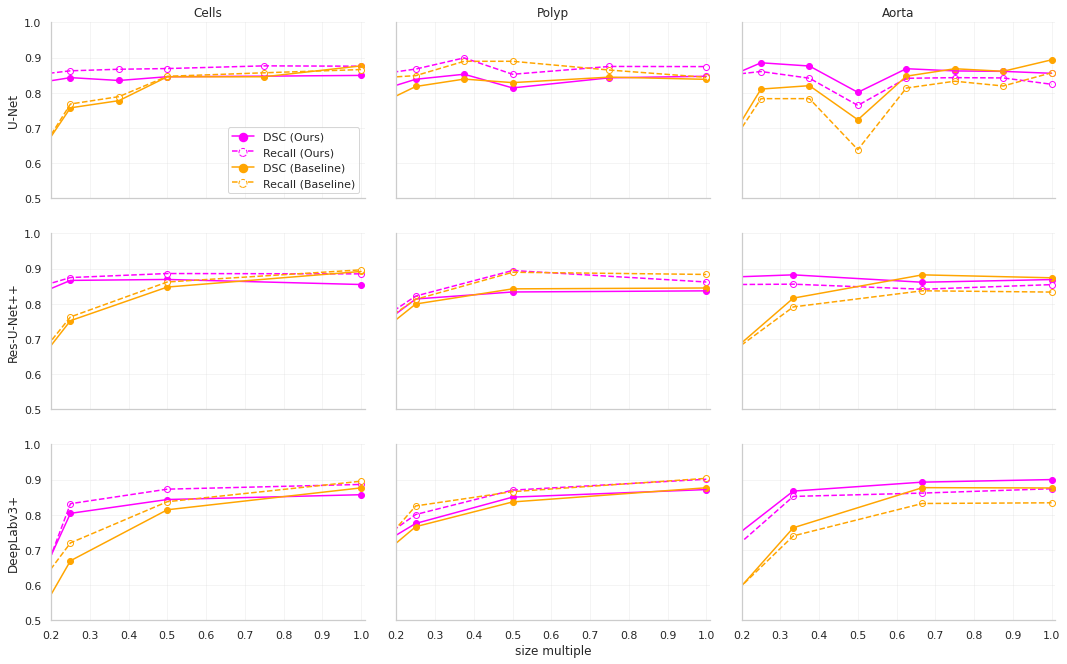
\includegraphics[width=\textwidth]{images/5/dsc-vs-size.png}
\caption{The relationship between input dimensions and the mean Dice Score Coefficient (DSC) and recall for different datasets. The points are measured values from our experiments. The Baseline model is trained on uniformly downscaled images.\label{fig:dsc-vs-size}}
\end{figure}

\begin{figure}[b!]
\centering
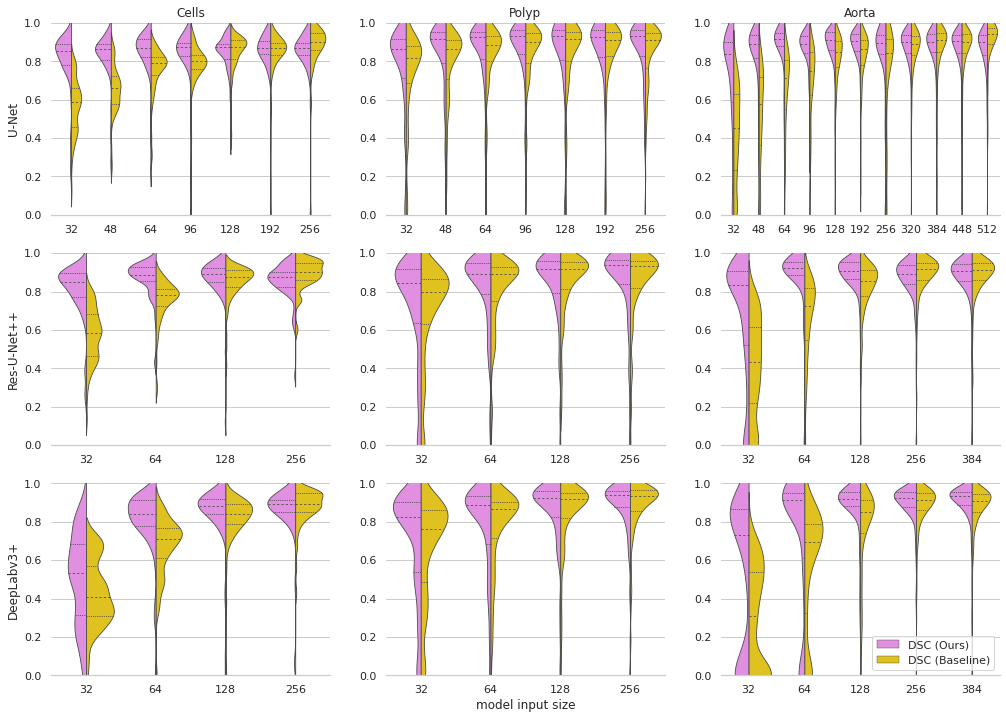
\includegraphics[width=\textwidth]{images/5/violin-plots.png}
\caption{Violin plots of Dice Score Coefficients of our approach compared to the baseline models trained on uniformly downscaled images at various input dimensions. The dashed lines represent quartiles of the distributions.\label{fig:box-plots}}
\end{figure}

The goal of our approach is increasing segmentation performance on downscaled images, so we do not expect a performance increase on the full-size images. While our approach offers significant improvements when using downscaled images, the main disadvantage of our approach is that it requires training two separate neural networks. However, this downside is lessened by two key factors. First, the cropped networks converge much faster since the objects are already localized and unified in scale in the images, making the problem easier for the network to learn. Secondly, since the architecture of the two networks is identical, one can use transfer learning from the trained rough segmentation network to the fine segmentation network.

\FloatBarrier

\subsubsection{Qualitative Assessment}

Qualitatively, there is a large improvement when using our approach over the baseline methods on downscaled inputs. At large downscaling factors, outputs from the baseline models often include artifacts on the border since the pixel grid is not fine enough to represent small variations on the object boundary. These issues disappear with our approach, as the overall downscaling amount is much lower. This effect is especially visible on the cells dataset due to its relatively small object size, as shown in Figure \ref{fig:examples-cells}. We observe a similar effect on the aorta dataset, shown in Figure \ref{fig:examples-aa}.

On the polyp dataset, our approach greatly reduces the number of false negative pixels on the image, as can be seen in Figure \ref{fig:examples-polyp}. U-Net fails to predict the whole polyp region on small input sizes, leading to ragged object boundaries and holes in the predicted regions. By comparison, our approach produces smoother, closed contours and manages to capture more of the object boundary than U-Net equivalents at the same input size.

\begin{figure}[b!]
	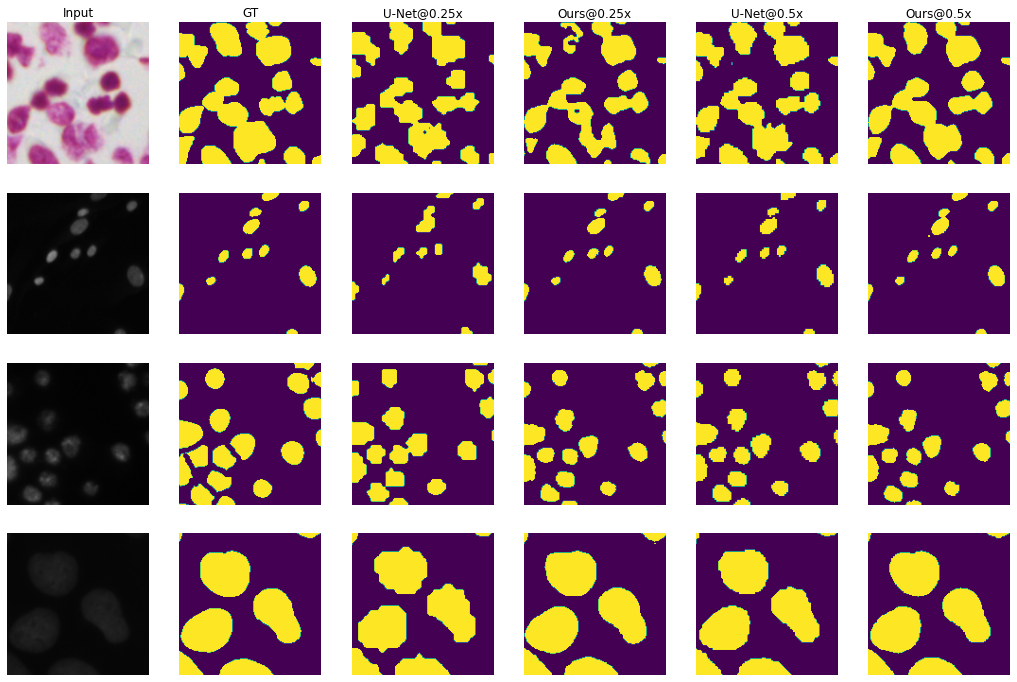
\includegraphics[width=\textwidth]{images/5/output_examples_cells.png}
	\caption{Example outputs from the models for the cells dataset at various input sizes. \cite{bencevicSegmentthenSegmentContextPreservingCropBased2023a}\label{fig:examples-cells}}
\end{figure}

\begin{figure}[t!]
	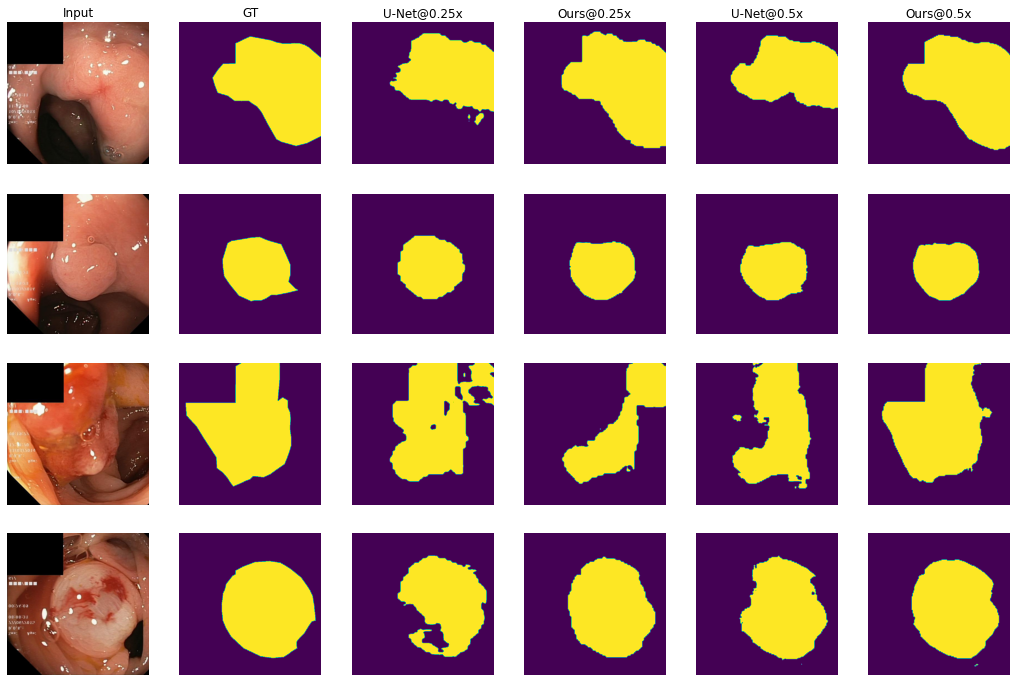
\includegraphics[width=\textwidth]{images/5/output_examples_polyp.png}
	\caption{Example outputs from the models for the polyp dataset at various input sizes. \cite{bencevicSegmentthenSegmentContextPreservingCropBased2023a}\label{fig:examples-polyp}}
\end{figure}

\begin{figure}[t!]
	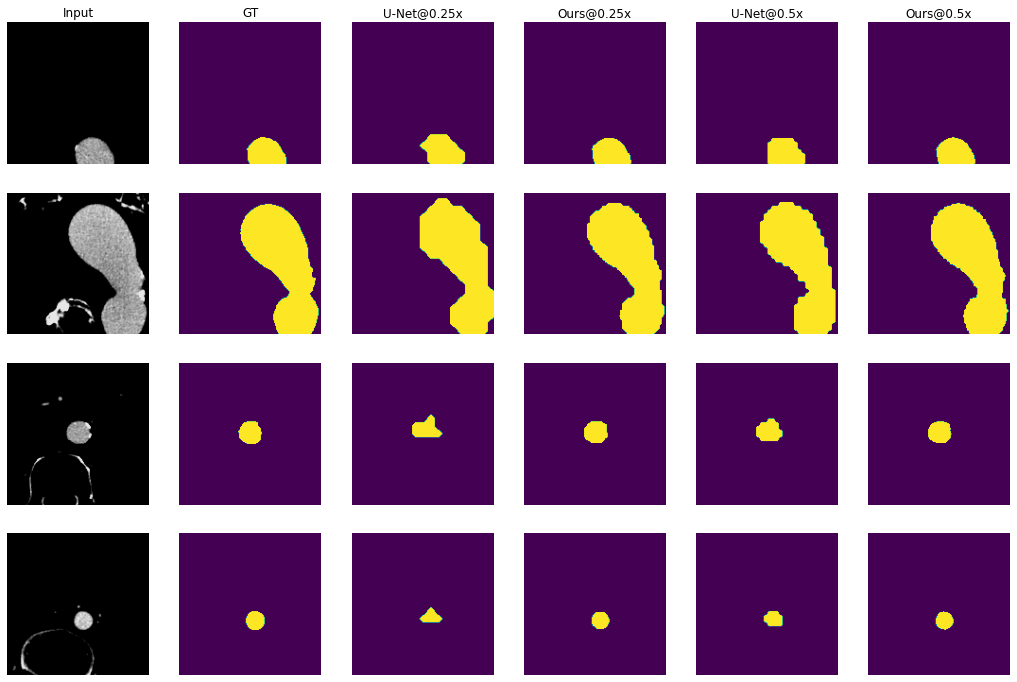
\includegraphics[width=\textwidth]{images/5/output_examples_aa.png}
	\caption{Example outputs from the models for the aorta dataset at various input sizes. \cite{bencevicSegmentthenSegmentContextPreservingCropBased2023a}\label{fig:examples-aa}}
\end{figure}

\FloatBarrier

\subsubsection{Computational Performance Characteristics}

Since our approach consists of using a cascade of two U-Nets, the number of parameters of the network is doubled. However, the peak GPU memory utilization during training and inference remains exactly the same when using our approach as with a baseline model on the same input size. Our approach allows one to reduce the input size while still maintaining the same segmentation metrics, thus allowing larger batch sizes during training. This is presented in Table \ref{tab:performance}.


\begin{table}[b!]
\caption{Performance characteristics of our approach compared to the baseline model with similar mean test Dice Score Coefficients.\label{tab:performance}}
		\newcolumntype{C}{>{\centering\arraybackslash}X}
		\begin{tabularx}{\textwidth}{lCCCCC}
			& \textbf{Input size} & \textbf{DSC} & \textbf{Peak VRAM$^{1, 3}$} & \textbf{Inf. time$^{2, 3}$} & \textbf{Max. batch size$^{3}$}\\
			\toprule
			\textbf{Cells} & & & & & \\
			\midrule
			U-Net & $64^2$ & 75.70 & 1.9 GB & 24 ms & $~300$\\
			Seg-Then-Seg & $64^2$ & 84.28 & 1.9 GB & 122 ms & $~300$\\
			U-Net & $128^2$ & 84.52 & 2.3 GB & 24 ms & $~80$\\
			
			\toprule
			\textbf{Polyp} & & & & & \\
			\midrule
			U-Net 		 & $48^2$ 	& 78.42 & 2.9 GB & 16 ms & $~850$\\
			Seg-Then-Seg & $48^2$ 	& 81.68 & 2.9 GB & 29 ms & $~850$\\
			U-Net 		 & $128^2$ 	& 82.86 & 3.8 GB & 16 ms & $~150$\\
						
			\toprule
			\textbf{Aorta} & & & & & \\
			\midrule
			U-Net 		 & $128^2$ 	& 81.03 & 2.9 GB  & 13 ms & $~46$\\
			Seg-Then-Seg & $128^2$ 	& 88.50 & 2.9 GB  & 26 ms & $~46$\\
			U-Net 		 & $512^2$ 	& 89.34 & 10.1 GB & 16 ms & $~9$\\
			\bottomrule
		\end{tabularx}
		\noindent{\footnotesize{\textsuperscript{1} Measured using a batch size of 8 for all rows.}} \\
		\noindent{\footnotesize{\textsuperscript{2} Mean inference time across all inputs in the test set, calculated per slice for the aorta dataset.}} \\
		\noindent{\footnotesize{\textsuperscript{3} Measured using PyTorch 1.10 on an Nvidia GeForce RTX 3080 GPU and an AMD Ryzen 7 3700x 8-core CPU with 32 GB of RAM.}}
\end{table}

In terms of computational performance, the largest downside of our approach is that it increases inference time non-linearly with the size of the images, which can be seen in Figure \ref{fig:inf-time}.

\begin{figure}[b!]
\centering
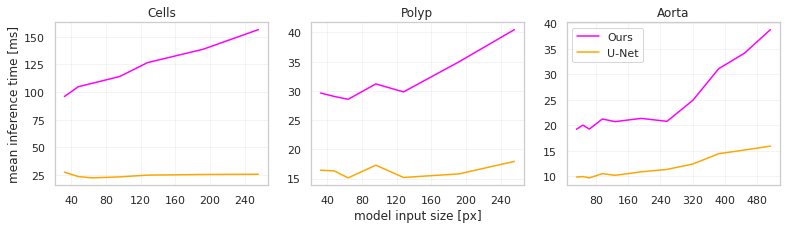
\includegraphics[width=\textwidth]{images/5/inf_time.png}
\caption{Mean per-input inference time across different input sizes for the U-Net-based models. \cite{bencevicSegmentthenSegmentContextPreservingCropBased2023a}\label{fig:inf-time}}
\end{figure}

This increase is explained by two key features of our approach. Firstly, cropping and rescaling operations take up a large percentage of the time. Secondly, each connected component in the initial segmentation is processed separately by the second network, thus inference time increases with the number of objects to be segmented. This is most apparent in the cells dataset, as the input images have the largest number of objects. Note that we use the implementation of \verb|torch.nn.functional.interpolate| with the nearest-neighbor mode in Pytorch 1.10 for all resizing. The inference time depends on the specific implementation of the resizing algorithm as well as the hardware it is being run on.

While these increases seem large in relative terms, it should be noted that in absolute terms the increases are in the order of magnitude of tens of milliseconds. We argue that such an increase in inference time does not limit the applicability of our approach in practical use cases.

Note that the goal of our method is not to produce state-of-the-art segmentation results on high-resolution images. Instead, the goal is to allow training on heavily downscaled images without sacrificing segmentation performance.

This initial version of the approach presents a promising avenue for future research. One way to improve the approach is to use a single end-to-end trainable network. We describe this kind of extension in the next section.

\section{An End-to-End Extension of Model-Driven Image Cropping}

So far, both in this chapter as well as the previous chapter, we employed separate networks for initial rough segmentation and subsequent fine segmentation. Instead of using separate neural networks, connecting the two networks end-to-end and training them as a single architecture presents distinct advantages. Training the rough and fine segmentation modules together could enhance the rough segmentation's ability to identify more accurate regions of interest, while the fine segmentation module could improve its robustness to imperfect initial segmentations.

A straightforward approach might involve chaining the two networks: an input image first undergoes rough segmentation, followed by fine segmentation of the transformed image, with both subnetworks trained simultaneously. This naive approach has several challenges. Firstly, since the network now needs to perform two segmentations, network convergence is much harder as there is no straightforward flow of gradients from the output to the input of the network. Secondly, the transformation procedure is potentially non-differentiable, and thus there could be no gradient calculated between the output layer of one subnetwork and the input layer of the other subnetwork.

To address these issues, we suggest two key modifications for a viable end-to-end model. Firstly, the output from the rough segmentation module is incorporated as an additional input channel to the fine segmentation module, facilitating gradient flow and providing context about the object's location. Secondly, we pre-train both subnetworks so they are already capable of segmenting images before they are fine-tuned together. This drastically reduces the chance that the end-to-end network will not converge. What follows is a more detailed description of the end-to-end network architecture.

\subsection{End-to-end Network Architecture and Training}

\begin{figure}[b!]
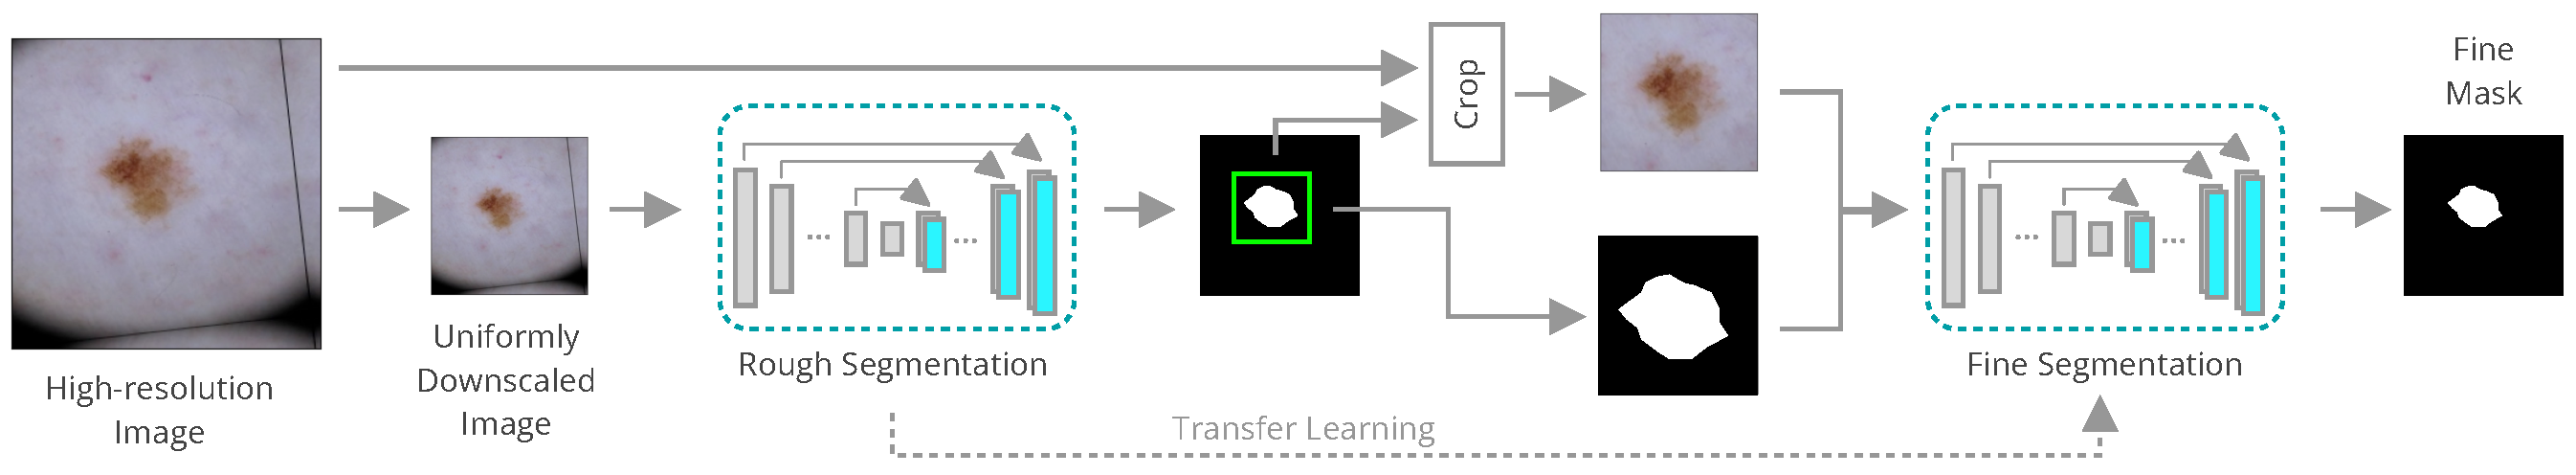
\includegraphics[width=\textwidth]{images/5/e2e/diagram.pdf}
\caption{An illustration of the end-to-end model-driven cropping architecture, comprising two interconnected modules: a coarse and a fine segmentation module, linked via a cropping layer. Both modules are designed to handle images of small, fixed input sizes. The first module processes a downscaled version of the input image. Its segmentation output determines the region of interest in the high-resolution image, which, along with the cropped initial segmentation, is fed into the fine segmentation module. Before being fine-tuned together, both networks are pre-trained as standard segmentation networks.\label{fig:e2e-diagram}}\end{figure}

As illustrated in \figref{fig:e2e-diagram}, the network consists of two stages, a coarse and fine segmentation stage, connected by a cropping layer. Both stages use the same U-Net-based segmentation architecture. The input size of each stage is fixed and smaller than the original image resolution. Assuming the input size of the network is $w \times h$, given a high-resolution input image $I'$ of size $W \times H$, we first uniformly downscale the image into $I$ of size $w \times h$ using linear interpolation. This image is then input into the coarse segmentation module producing a segmentation mask $M_{coarse}(I)$.

The segmentation mask $M_{coarse}$ is then upscaled to $M'_{coarse}$ of size $W \times H$ and thus matches the high-resolution image. Then, a bounding box is calculated such that it encompasses all non-zero regions of $M'_{coarse}$ and expanded by 20 pixels in each direction, clipped to the bounds of the image. The bounding box is used to crop $I'$ and the crop is then scaled to $w \times h$, producing a high-resolution input region of interest $I_{crop}$. Note that scaling the crop region to $w \times h$ results in a much lower total scaling than it does when scaling down the whole image. In cases where $M_{coarse}$ has no non-zero pixels, the bounding box is set to the whole image, i.e. $I_{crop} = I$. From our experiments, such cases are exceedingly rare.

Then, an input vector is constructed for the fine segmentation network as $x_{fine} = [I_{crop}, M_{coarse}]$ --- in other words, the first channel is the high-resolution crop, while the second channel is the coarse segmentation mask. The fine segmentation network then produces a final segmentation mask $M(x_{fine})$ which is used as the output of the whole model.

We use pre-training to allow the two networks to reliably converge. First, we train a regular segmentation network on uniformly downscaled images $I$. Once trained, the weights of this model are transferred both to the rough and fine segmentation modules of our proposed network architecture.

\subsection{Experiments in Clinical Dermatological Image Segmentation}

We validate this end-to-end architecture on segmenting the skin lesion boundary in clinical dermatological images using datasets of small sample sizes. Namely, we use the University of Waterloo skin cancer database \cite{waterloo} (available at \cite{uwaterlooSkinCancer}) of clinical skin lesion images. The dataset consists of manual segmentation labels of two publicly available skin lesion databases, DermIS \cite{dermisDermIS} (69 images) and DermQuest (137 images, no longer available). We treat these two collections as two different centers to evaluate out-of-sample performance. The images are of various sizes from 300 to 550 pixels in height and width. As a preprocessing step, each image of each dataset is normalized to $[-0.5, 0.5]$.

We use PyTorch 1.10 for all experiments. All models are trained on an Nvidia GeForce RTX 3080. Wherever possible, we fix an arbitrarily chosen random seed value of ``2022'' to increase reproducibility. We use the Adam optimizer for all training while reducing the learning rate on plateaus by a factor of 0.1. The best model is selected and saved during training based on validation loss. We use a learning rate of $10^{-4}$ for both pre-training and fine-tuning. We set the batch size to 16 for all input sizes except $512 \times 512$, where the batch size was set to 4. The aforementioned hyperparameters were chosen based on the validation DSC of the models. For ease of implementation, all high-resolution input images are resized to $1024 \times 1024$ pixels, but this is not a required step for our method, which can work with any high-resolution input image size.

\subsubsection{Results and Discussion}

To evaluate our method, we train a baseline U-Net model and our end-to-end image-cropping approach for input sizes $64 \times 64$, $128 \times 128$, $256 \times 256$, and $512 \times 512$. The same architecture was used for the baseline U-Net model as well as for the rough and fine segmentation modules in our method. We employed 5-fold cross-validation to evaluate in-sample performance, resulting in five distinct models for each dataset. For out-of-sample performance evaluation, each image in one dataset was segmented using the five models trained on the other dataset. Segmentation metrics were calculated for each prediction and then averaged, ensuring that all reported out-of-sample metrics represent an average from models trained across five different data splits.

The two segmentation metrics we use for the evaluation are the Dice Similarity Coefficient (DSC) as well as the Thresholded Jaccard Index. DSC takes into account both the accuracy and recall of the method and is thus a good general segmentation metric. The Thresholded Jaccard Index was proposed for lesion segmentation in the ISIC 2018 challenge \cite{codellaSkinLesionAnalysis2018} to account for specific needs in skin lesion segmentation. Low-accuracy segmentations (in this case defined as those with a Jaccard Index less than 0.65) are not useful for further lesion analysis. Therefore, instead of a simple mean result calculation, all results with a Jaccard Index below 0.65 are set to zero. This has been shown to better represent true segmentation performance in the context of lesion segmentation. 

Visually, our approach demonstrates enhanced performance in delineating lesion boundaries, as evident in Figure \ref{fig:visual}. The segmentation results more accurately adhere to the ground truth contours and exhibit fewer false-positive regions compared to those generated by the baseline models.

\begin{figure}[t!]
\centering
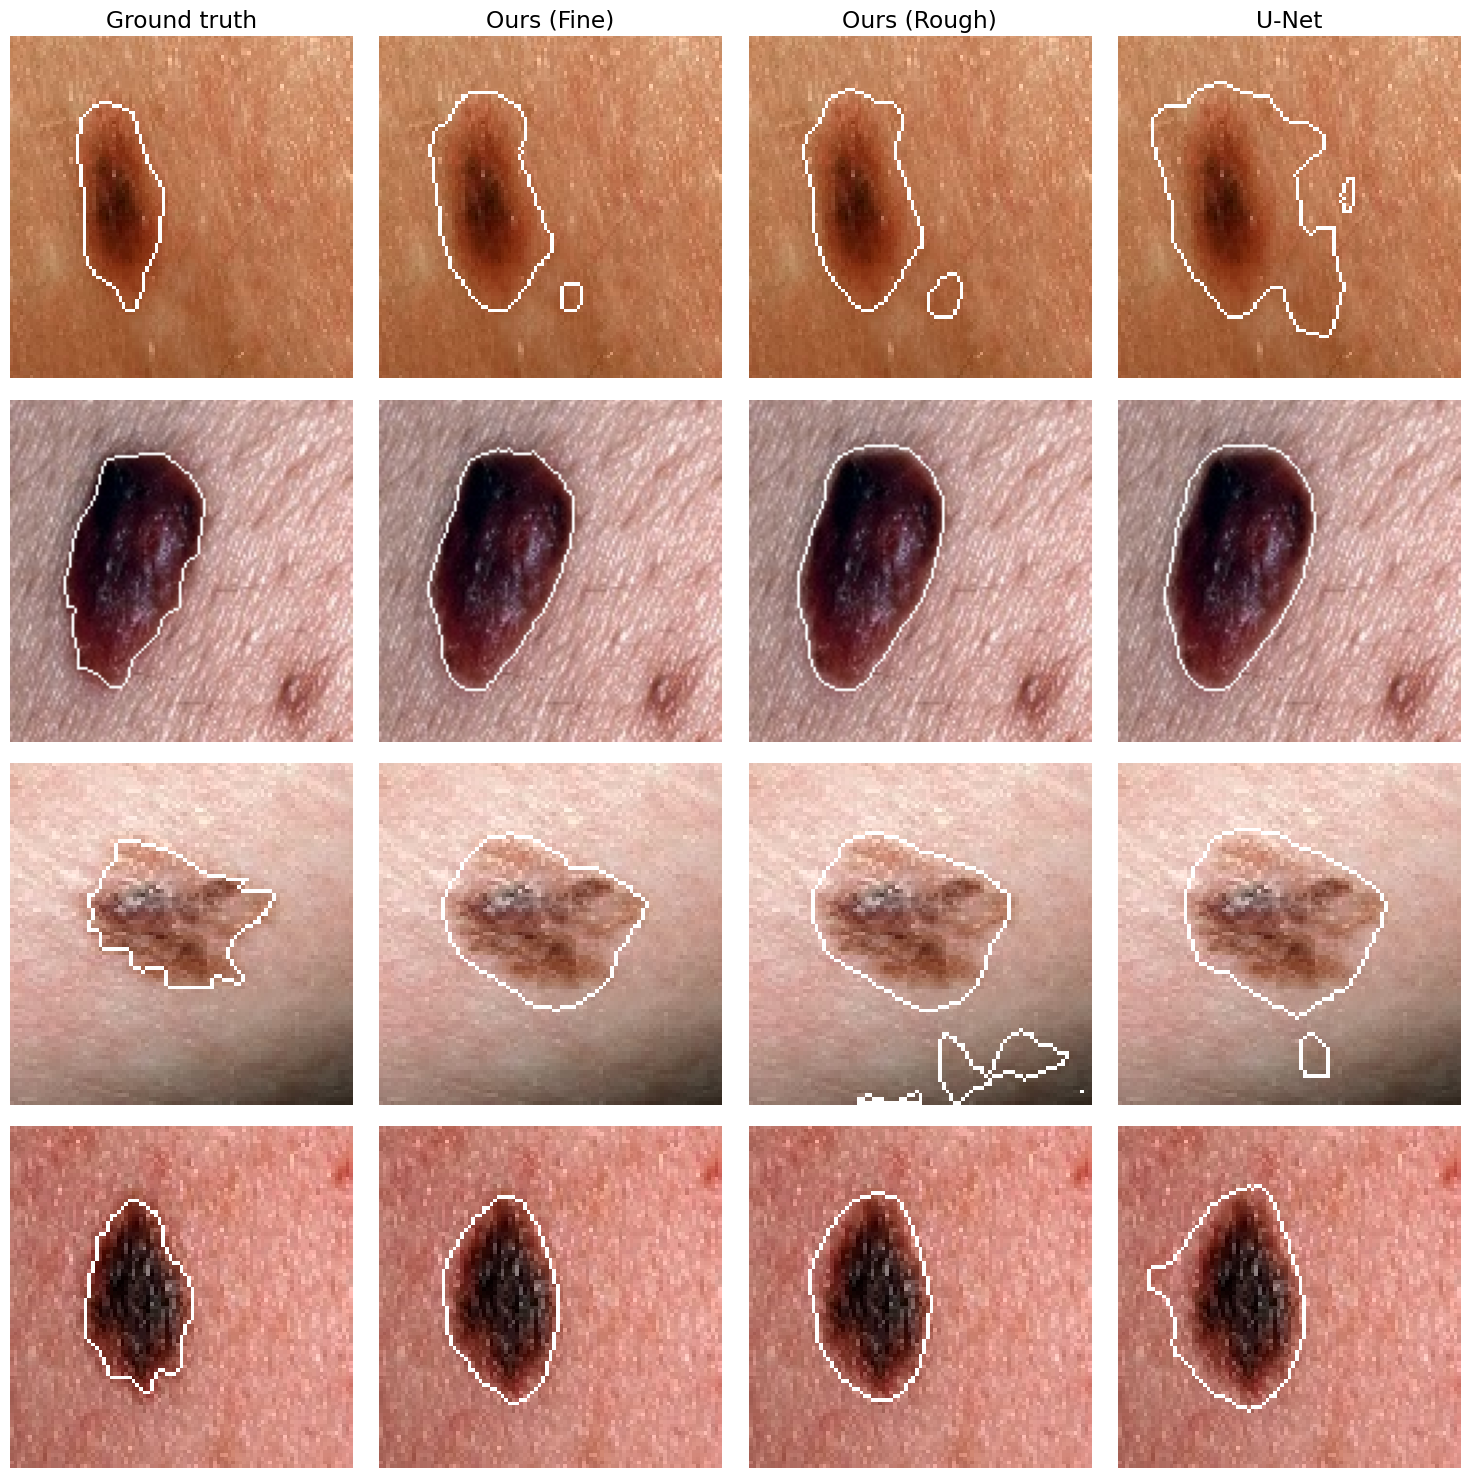
\includegraphics[width=\textwidth]{images/5/e2e/visual_results.png}
\caption{Randomly chosen examples of out-of-sample segmentation results. The columns, from left to right, show the input image with the ground truth segmentation mask, the final output segmentation mask of our approach, the rough segmentation of our approach, and the output of a baseline U-Net model. The images are zoomed in on the lesion region.} \label{fig:visual}
\end{figure}

Quantitatively, in-sample and out-of-sample results of our model compared to a baseline U-Net are shown in Table \ref{tab:results}. When comparing our method and a baseline U-Net using the same input size, we note an increase in DSC in almost all experiments. We see similar results for the Thresholded Jaccard Index. These increases can give us an estimate of how much we can reduce the input size of an image while still retaining the same segmentation quality. For instance, using our approach, we can go from $256 \times 256$ to $64 \times 64$ images while achieving the same in-sample as well as out-of-sample Thresholded Jaccard Index for DermIS.

\begin{table}[t!]
\caption{Results of our approach and the baseline model in terms of the Dice Coefficient (DSC) as well as the thresholded Jaccard index (Th. Jacc.) for various experiments. Results are shown in the form of mean $\pm$ standard deviation. The top two groups show in-sample performance within the DermIS and DermQuest datasets, while the bottom two groups show out-of-sample performance when trained on DermIS and tested on DermQuest, and vice-versa.}\label{tab:results}
\def\arraystretch{1.2}
\setlength\tabcolsep{1em}
\begin{tabularx}{\textwidth}{X|cc|cc}
& \multicolumn{2}{c|}{U-Net} & \multicolumn{2}{c}{Ours} \\
\midrule
 \textbf{Size}                                                     & \textbf{DSC}           & \textbf{Th. Jacc.}     & \textbf{DSC}           & \textbf{Th. Jacc.}     \\
\midrule
 &\multicolumn{4}{c}{DermIS}                         \\
\midrule
 64                                                       & 85.51 $\pm$ 15.50 & 70.31 $\pm$ 31.38 & 87.01 $\pm$ 15.06 & 74.57 $\pm$ 27.97 \\
 128                                                      & 86.53 $\pm$ 15.71 & 72.21 $\pm$ 30.78 & 88.82 $\pm$ 11.93 & 75.84 $\pm$ 28.41 \\
 256                                                      & 88.09 $\pm$ 14.58 & 73.58 $\pm$ 33.01 & 89.88 $\pm$ 12.49 & 77.04 $\pm$ 30.77 \\
 512                                                      & 89.85 $\pm$ 16.90 & 81.32 $\pm$ 26.32 & 90.35 $\pm$ 17.07 & 83.40 $\pm$ 24.35 \\
 \midrule
 &\multicolumn{4}{c}{DermQuest}                      \\
\midrule
 64                                                       & 87.75 $\pm$ 9.07  & 71.61 $\pm$ 29.56 & 87.83 $\pm$ 8.97  & 73.96 $\pm$ 25.84 \\
 128                                                      & 88.83 $\pm$ 10.19 & 76.59 $\pm$ 25.76 & 89.45 $\pm$ 10.09 & 77.93 $\pm$ 25.00 \\
 256                                                      & 89.61 $\pm$ 11.20 & 77.34 $\pm$ 27.73 & 90.10 $\pm$ 11.22 & 78.99 $\pm$ 26.18 \\
 512                                                      & 91.14 $\pm$ 9.18  & 81.31 $\pm$ 23.69 & 90.52 $\pm$ 12.98 & 81.16 $\pm$ 24.76 \\
\midrule
 &\multicolumn{4}{c}{DermIS $\rightarrow$ DermQuest} \\
\midrule
 64                                                       & 77.11 $\pm$ 13.58 & 43.40 $\pm$ 34.37 & 80.94 $\pm$ 12.85 & 54.56 $\pm$ 31.45 \\
 128                                                      & 80.20 $\pm$ 12.92 & 50.81 $\pm$ 33.87 & 79.61 $\pm$ 14.15 & 52.46 $\pm$ 32.36 \\
 256                                                      & 78.67 $\pm$ 15.32 & 51.10 $\pm$ 33.30 & 80.07 $\pm$ 14.55 & 55.18 $\pm$ 31.51 \\
 512                                                      & 80.96 $\pm$ 14.38 & 60.73 $\pm$ 26.96 & 83.34 $\pm$ 13.29 & 66.72 $\pm$ 24.61 \\
\midrule
 &\multicolumn{4}{c}{DermQuest $\rightarrow$ DermIS} \\
\midrule
 64                                                       & 78.94 $\pm$ 18.81 & 54.98 $\pm$ 34.36 & 81.85 $\pm$ 17.24 & 60.87 $\pm$ 32.66 \\
 128                                                      & 78.31 $\pm$ 19.36 & 51.57 $\pm$ 37.63 & 81.51 $\pm$ 18.23 & 60.10 $\pm$ 35.86 \\
 256                                                      & 81.10 $\pm$ 19.54 & 60.81 $\pm$ 35.41 & 81.97 $\pm$ 19.46 & 63.12 $\pm$ 34.89 \\
 512                                                      & 83.60 $\pm$ 18.73 & 65.59 $\pm$ 32.99 & 82.82 $\pm$ 19.70 & 64.50 $\pm$ 33.35 \\
\end{tabularx}
\end{table}

The thresholded Jaccard index assumes that any segmentation with a Jaccard index below 0.65 is a failed segmentation, i.e. it cannot be used for any downstream analysis of the legion due to its insufficient accuracy. Consequently, we examined the frequency of these failed segmentations across various input sizes, as depicted in Figure \ref{fig:box-plot}. The findings indicate a general improvement in the mean Jaccard Index (exceeding 0.65) when utilizing our model, particularly for smaller input sizes, and this trend persists even in out-of-sample evaluations. Additionally, there is a noticeable decrease in the incidence of failed segmentations (Jaccard Index < 0.65) in all but two experiments. This decline is most pronounced with smaller input sizes, suggesting that our method significantly enhances the robustness of segmentations derived from images with small input sizes.

\begin{figure}[t!]
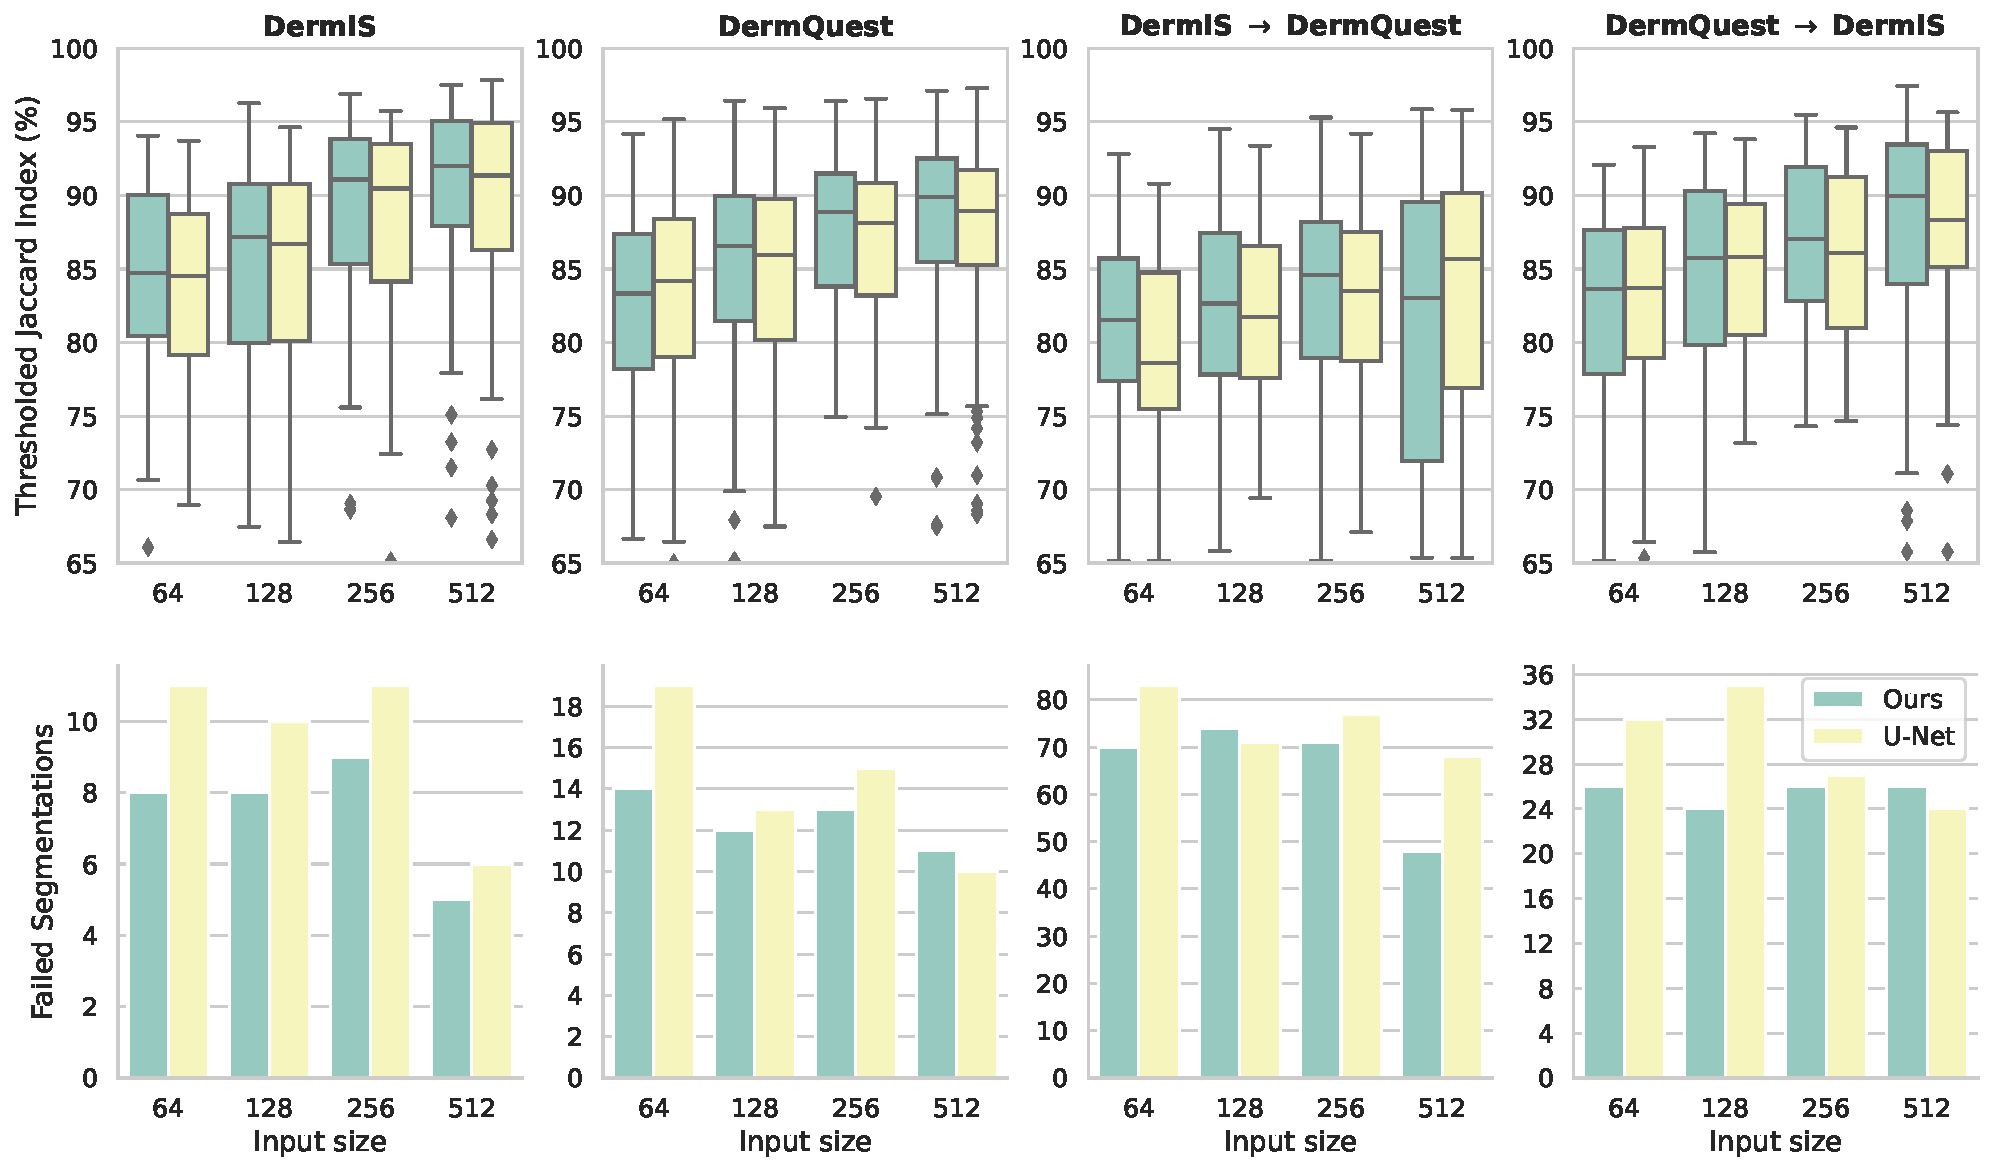
\includegraphics[width=\textwidth]{images/5/e2e/boxplots.pdf}
\caption{A box plot of Jaccard indices above or equal to 0.65 (above) and the number of Jaccard indices below 0.65 (below). The first two columns show in-sample results, while the last two columns show out-of-sample results for models trained on DermIS and tested on DermQuest and vice-versa.} \label{fig:box-plot}
\end{figure}

\clearpage

\section{Conclusion}

Downscaling is a common source of segmentation errors in neural networks. In this chapter, we presented an approach to training neural networks that reduces downscaling by utilizing two neural networks and salient crops. We show how training a second neural network on cropped image regions can improve segmentation performance on small input sizes with few downsides. Our approach improves segmentation metrics on downscaled images across different modalities and image sizes, especially in terms of recall. We show that, while this approach increases inference time, it allows for training using much larger batch sizes while maintaining the same segmentation metrics. By utilizing transfer learning, we successfully addressed issues related to network convergence and provided an end-to-end extension of this method. Using our approach, we were able to reduce input sizes by at least half while retaining the same segmentation quality.

A significant advantage of our approach is the reduced requirement for detailed segmentation labels in the rough segmentation stage. This stage only necessitates approximate object localization, achievable through simpler, potentially unsupervised methods like heuristic-based and traditional image processing techniques. Moreover, one can use weakly supervised training using pseudo-labels, instead of segmentation masks. While we did not evaluate our approach on 3D networks in this chapter, there is nothing in our approach that is specific to 2D images. Our approach can be extended to 3D images by using 3D neural network architectures and 3D bounding boxes for crop regions.

However, our approach has certain limitations. Notably, from our experiments in datasets with large sample sizes, our method did not substantially improve segmentation quality. We speculate that our approach acts as a form of regularization, beneficial in scenarios where overfitting is a concern due to small sample sizes and high-capacity networks. This regularization may be redundant in cases with ample sample sizes. Nonetheless, the primary aim of our approach is to improve data efficiency in terms of both input size and sample size.

We believe that this method can be broadly applied to enhance segmentation performance and robustness in a variety of image segmentation challenges, particularly where object scale and location variance are significant and the sample size is small. The methods presented in this chapter were published in \cite{bencevicSegmentthenSegmentContextPreservingCropBased2023a} and \cite{bencevicCropGuidedNeuralNetwork2024}.


 